

\tikzset{every picture/.style={line width=0.75pt}} %set default line width to 0.75pt        

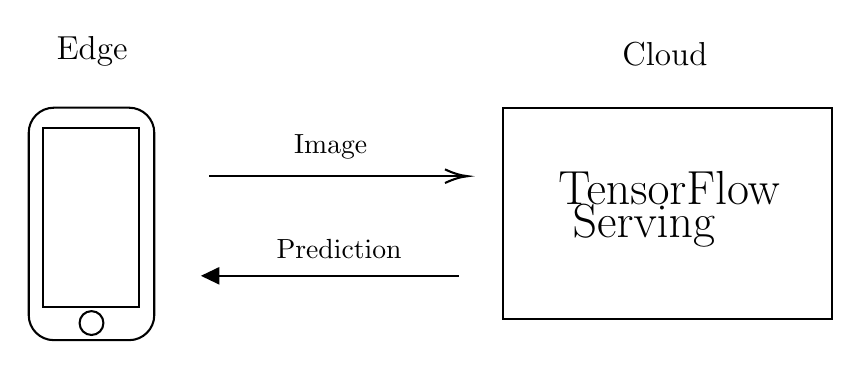
\begin{tikzpicture}[x=0.75pt,y=0.75pt,yscale=-1,xscale=1]
%uncomment if require: \path (0,300); %set diagram left start at 0, and has height of 300

\draw   (69.5,176) -- (115.5,176) -- (115.5,262) -- (69.5,262) -- cycle ;
\draw   (62.5,178.1) .. controls (62.5,171.42) and (67.92,166) .. (74.6,166) -- (110.9,166) .. controls (117.58,166) and (123,171.42) .. (123,178.1) -- (123,265.9) .. controls (123,272.58) and (117.58,278) .. (110.9,278) -- (74.6,278) .. controls (67.92,278) and (62.5,272.58) .. (62.5,265.9) -- cycle ;
\draw   (87,269.75) .. controls (87,266.57) and (89.57,264) .. (92.75,264) .. controls (95.93,264) and (98.5,266.57) .. (98.5,269.75) .. controls (98.5,272.93) and (95.93,275.5) .. (92.75,275.5) .. controls (89.57,275.5) and (87,272.93) .. (87,269.75) -- cycle ;
\draw    (149.48,199) -- (272,199) ;
\draw [shift={(274,199)}, rotate = 540] [color={rgb, 255:red, 0; green, 0; blue, 0 }  ][line width=0.75]    (10.93,-3.29) .. controls (6.95,-1.4) and (3.31,-0.3) .. (0,0) .. controls (3.31,0.3) and (6.95,1.4) .. (10.93,3.29)   ;

\draw    (147.48,247) -- (270,247) ;

\draw [shift={(145.48,247)}, rotate = 360] [fill={rgb, 255:red, 0; green, 0; blue, 0 }  ][line width=0.75]  [draw opacity=0] (8.93,-4.29) -- (0,0) -- (8.93,4.29) -- cycle    ;
\draw   (291,166) -- (449.5,166) -- (449.5,268) -- (291,268) -- cycle ;

\draw (208,185) node  [align=left] {Image};
\draw (212,234) node  [align=left] {Prediction};
\draw (93,139) node  [align=left] {{\large Edge}};
\draw (369,140) node  [align=left] {{\large Cloud}};
\draw (371,215) node  [align=left] {{\LARGE TensorFlow}\\{\LARGE  \  Serving}};


\end{tikzpicture}